% Этот шаблон документа разработан в 2017 году
% Владимиром Коротковым (kvamob@mail.ru) 
%  

\documentclass[a4paper,12pt]{article} % добавить leqno в [] для нумерации слева

%% Глобальные Параметры страницы
%\usepackage[left=3cm,right=2cm,top=1cm,bottom=2cm,bindingoffset=0cm]{geometry}

%\usepackage{fp} 						% Вычисления с плавающей точкой
%\usepackage{siunitx}					% При использовании пакета fp все числа должны иметь decimal delimiter точку
%\sisetup{output-decimal-marker={,}}		% Числа выводятся с запятой в качестве разделителя разрядов: \num{3.2} выводит 3,2 

%%% Работа с русским языком
\usepackage{cmap}					% поиск в PDF
\usepackage{mathtext} 				% русские буквы в формулах
\usepackage[T2A]{fontenc}			% кодировка
\usepackage[utf8]{inputenc}			% кодировка исходного текста
\usepackage[english,russian]{babel}	% локализация и переносы

%%% 
%\usepackage{rotating}				% Поворот текста

%%% Дополнительная работа с математикой
\usepackage{amsmath,amsfonts,amssymb,amsthm,mathtools} % AMS
\usepackage{icomma} % "Умная" запятая: $0,2$ --- число, $0, 2$ --- перечисление

%% Номера формул
%\mathtoolsset{showonlyrefs=true} % Показывать номера только у тех формул, на которые есть \eqref{} в  тексте.

%% Шрифты
\usepackage{euscript}	 % Шрифт Евклид
\usepackage{mathrsfs} % Красивый матшрифт


%% Перенос знаков в формулах (по Львовскому)
% \newcommand*{\hm}[1]{#1\nobreak\discretionary{}
%	{\hbox{$\mathsurround=0pt #1$}}{}}

%%% Работа с картинками
\usepackage{graphicx}  % Для вставки рисунков
%\usepackage[export]{adjustbox}
\graphicspath{{images/}{images2/}}  % папки с картинками
\setlength\fboxsep{3pt} % Отступ рамки \fbox{} от рисунка
\setlength\fboxrule{0.2pt} % Толщина линий рамки \fbox{}
\usepackage{wrapfig} % Обтекание рисунков и таблиц текстом


%%% Работа с таблицами
\usepackage{array,tabularx,tabulary,booktabs} % Дополнительная работа с таблицами
\usepackage{longtable}  % Длинные таблицы
\usepackage{multirow} % Слияние строк в таблице

%\usepackage{caption} % подписи к рисункам в русской типографской традиции
%\DeclareCaptionFormat{GOSTtable}{#2#1\\#3}
%\DeclareCaptionLabelSeparator{fill}{\hfill}
%\DeclareCaptionLabelFormat{fullparents}{\bothIfFirst{#1}{~}#2}
%\captionsetup[table]{
%	format=GOSTtable,
%	font={footnotesize},
%	labelformat=fullparents,
%	labelsep=fill,
%	labelfont=rm,
%%	labelfont=it,
%	textfont=bf,
%	justification=centering,
%	singlelinecheck=false
%}

%%%%%%%%%%%%%%%%%%%%%%%%%%%%%%%%%%%%%%%%%%%%%%%%%%%%%%%%%%%%%%%%%%%%%%%%%%%%%%%%%%%%%%%%%%%%%%%%%%%%%%%%%
%%% PAYLOAD
%%%%%%%%%%%%%%%%%%%%%%%%%%%%%%%%%%%%%%%%%%%%%%%%%%%%%%%%%%%%%%%%%%%%%%%%%%%%%%%%%%%%%%%%%%%%%%%%%%%%%%%%%

%%% Заголовок
\author{ООО <<Гидросфера>>}\label{company}
\title{ОТЧЕТ ПО РЕЗУЛЬТАТАМ РАСЧЕТА ДРЕНАЖНОЙ СИСТЕМЫ}
\date{\today}
%%%======================================================================================================
\newcommand{\txtExecutor}{ООО <<Гидросфера>>}	% Исполнитель
\newcommand{\txtYear}{2017}						% Год
\newcommand{\txtAddress}{--Address--}			% Адрес
\newcommand{\txtCadaster}{--Cadaster--} 		% Кадастровый номер


%%%%%%%%%%%%%%%%%%%%%%%%%%%%%%%%%%%%%%%%%%%%%%%%%%%%%%%%%%%%%%%%%%%%%%%%%%%%%%%%%%%%%%%%%%%%%%%%%%%%%%%%%

\begin{document} % конец преамбулы, начало документа

\setlength{\extrarowheight}{1mm} % Дополнительный интервал между строками таблиц

%% Титульная страница

\begin{titlepage}
	\begin{center}
		\textbf{\txtExecutor}
		\vspace{5.5cm}
		
		{\LARGE ОТЧЕТ ПО РЕЗУЛЬТАТАМ РАСЧЕТА ДРЕНАЖНОЙ СИСТЕМЫ}
		\vspace{0.25cm}
		
		\bigskip
		
		на участке по адресу:
				
		\underline{\txtAddress}
		
		\bigskip
		Кадастровый номер \txtCadaster
		
		\vfill
	
		\bigskip
		
	\end{center}

	\vfill
	
	\newlength{\ML}
	\settowidth{\ML}{«\underline{\hspace{0.7cm}}» \underline{\hspace{2cm}}}
	\hfill
	\begin{minipage}{1.0\textwidth}
		Директор ООО <<Гидросфера>> к.г.м.н.
		\underline{\hspace{\ML}} А.\,А.~Кашкаров\\
	\end{minipage}%
	
	\bigskip
	
	\vfill
	\begin{center}
		Екатеринбург, \txtYear
	\end{center}			

	\end{titlepage}

%%%%%%%%%%%%%%%%%%%%%%%%%%%%%%%%%%%%%%%%%%%%%%%%%%%%%%%%%%%%%%%%%%%%%%%%%%%%%%%%

\section{Введение}

На исследуемой территории, на которой расположен жилой дом с подвальным помещением, наблюдаются явления подтопления. При разработке плана мероприятий по водопонижению было изучено геологическое строение участка и учитывались следующие требования:
\begin{itemize}
\item Водопонижение должно осуществляться непрерывно;
\item При устройстве дренажных сооружений повреждения верхнего естественного покрова должны быть минимальными.
\end{itemize}

\section{Геологические, гидрогеологические условия площадки и причины подтопления}

Рассматриваемый участок расположен в районе экзоконтакта гранитного массива и сложен зелеными сланцами, амфиболитами. Скальные грунты перекрыты мезозойской корой выветривания, представленной преимущественно суглинками и глинами, образующими водоупорные линзы, на которых формируются временные горизонты приповерхностных подземных вод («верховодка»). Глубина залегания первого устойчивого горизонта подземных вод превышает 15 м.

\textbf{В гидрогеологическом отношении} рассматриваемый участок расположен в пределах Большеуральского сложного бассейна корово - блоковых напорных и безнапорных вод, в области развития палеозойских метаморфических горных пород. С поверхности палеозойские породы на отдельных участках перекрыты спорадически распространенной щебнисто - глинистой корой выветривания и повсеместно - четвертичными отложениями мощностью от первых метров до 5 - 8 м. Подземные воды приурочены к зоне трещиноватости палеозойских интрузивных пород мощностью 40 - 50 м, а в зонах тектонических нарушений и литологических контактов -- до 70 - 80 м. 

Зеркало подземных вод в сглаженном виде повторяет формы рельефа поверхности. Глубина залегания уровня – свыше 15 м. Так как мощность перекрывающих слабо водопроницаемых отложений не выдержана в плане и разрезе, подземные воды недостаточно защищены от поверхностного загрязнения.

По химическому составу подземные воды рассматриваемого района в природных условиях относятся к типу гидрокарбонатных кальциево-магниевых с минерализацией до 0,3 г/дм\textsuperscript{3}, жесткостью 2 - 3 ммоль/дм\textsuperscript{3}. Современное качество воды в условиях интенсивной техногенной нагрузки этой территории претерпело изменения в связи с увеличением в солевом составе воды доли хлоридов и сульфатов. Общая минерализация варьирует в пределах 0,3 - 0,5 г/дм\textsuperscript{3}.

Залегание уровня подземных вод ожидается на глубине свыше 15 м.

В геоморфологическом отношении участок расположен в восточной прибрежной части озера Шарташ. Поверхностный и подземный поток от этого участка направлен в западном направлении в котловину оз. Шарташ.

Осложняющим фактором, вызывающим подтопление на изучаемом участке, является наличие в разрезе водонепроницаемых грунтов, сложная форма кровли суглинков и глин коры выветривания и коренных грунтов, застройка окружающей территории, что вызывает неравномерный напор приповерхностных вод. Источником приповерхностных вод на изучаемом участке являются преимущественно атмосферные осадки и воды, образующиеся в периоды сезонного снеготаяния.

Поскольку устойчивые горизонты подземных вод залегают на глубинах свыше 15\-м, \underline{основной причиной подтопления} является отсутствие сброса собранной ливневыми желобами воды и вследствие этого, накопление ее в приповерхностных грунтах и дальнейшее ее поступление в подвальные помещения.

\section{Обоснование выбора типа дренажных мероприятий}

Учитывая гидрогеологические условия площадки и требования к системе дренажа, был выбран вариант вертикального дренажа, представляющего собой серию из 3 водопоглощающих дренажных скважин глубиной 30 м каждая, расположенных по линии вдоль одной из стен здания (Приложение 3). 

Данные скважины работают как дренажно-поглощающие трубчатые колодцы - по их стволам приповерхностные воды фильтруются в водопроницаемые трещиноватые грунты, залегающие под  водоупорным горизонтом суглинков (рис. \ref{img:scheme1}). За счет взаимного влияния депрессионных воронок снимаются неравномерности напора приповерхностных вод и локальные области переувлажнения несущих грунтов ликвидируются.

\begin{figure}[!h]
	\centering
	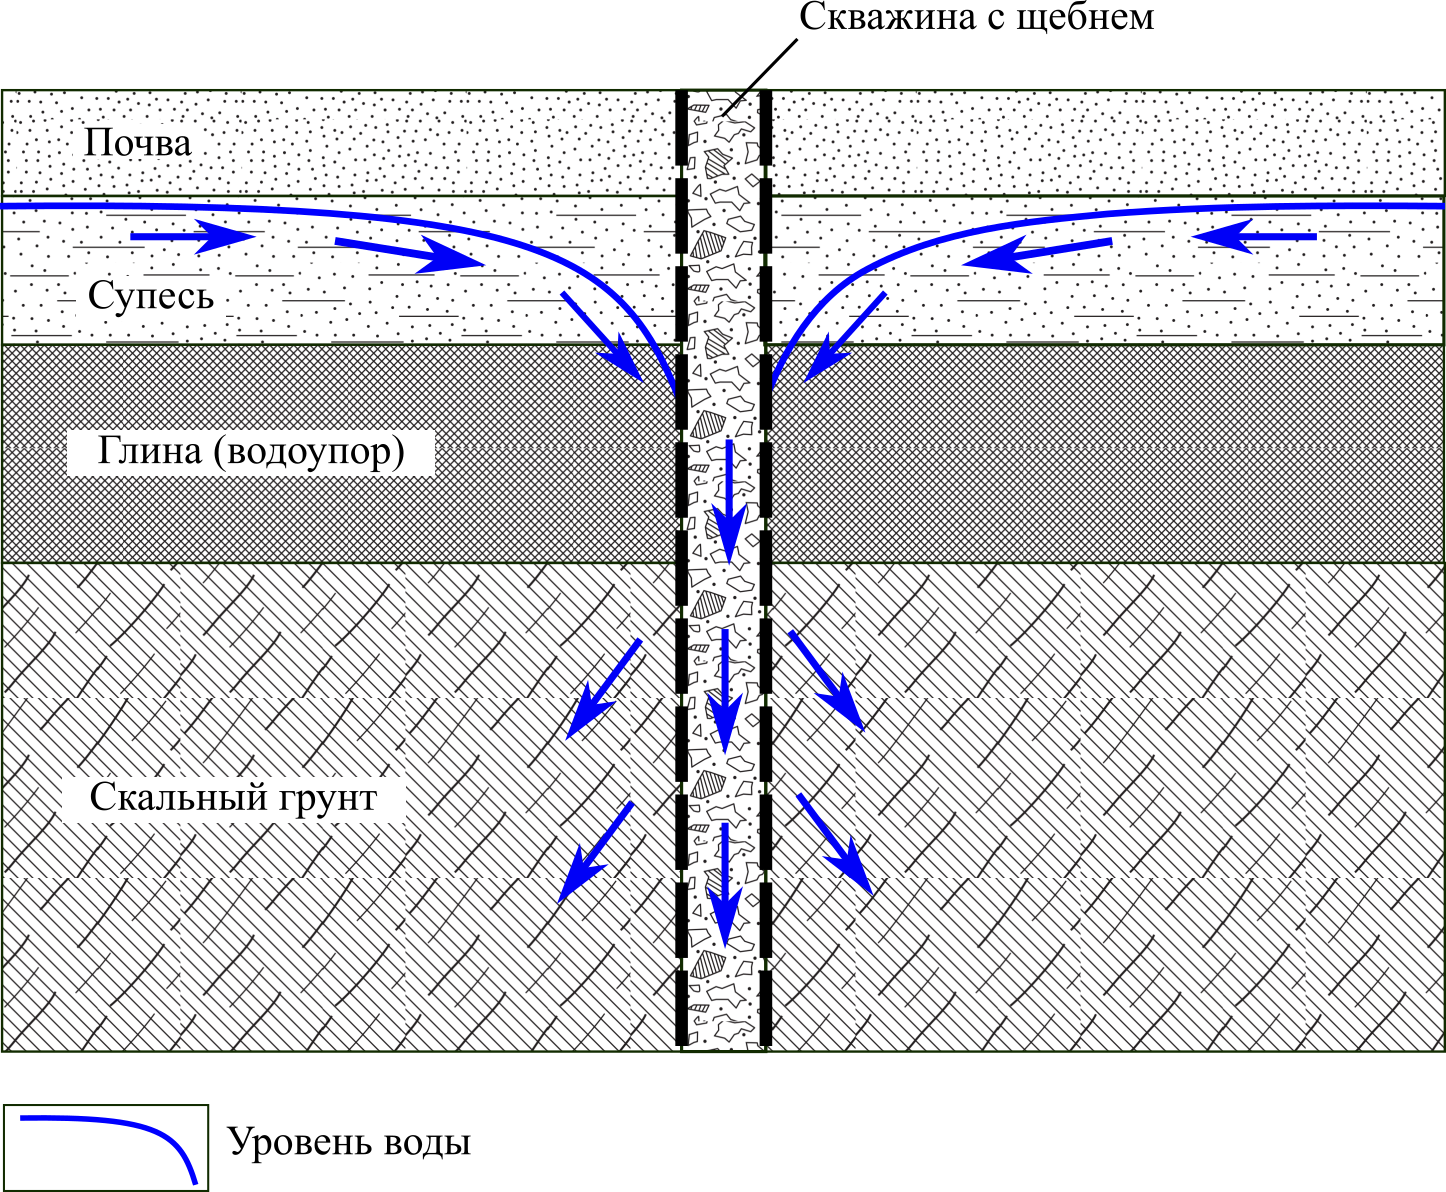
\includegraphics{img1.png}
	\caption[Схема водопонижения]{Схема водопонижения – воды, залегающие на водоупоре, по дренирующей скважине спускаются в трещиноватые скальные грунты}
	\label{img:scheme1}
\end{figure}

Бурение необходимо проводить с обсадными трубами, после проходки каждой скважины на проектную глубину ствол засыпается щебнем, а трубы вынимаются. 
В устье каждой скважины устраивается дренажный колодец, соединяемый с ливневыми желобами. Дренажные колодцы засыпаются щебнем и закрываются крышками.

\begin{figure}[!h]
	\centering
%	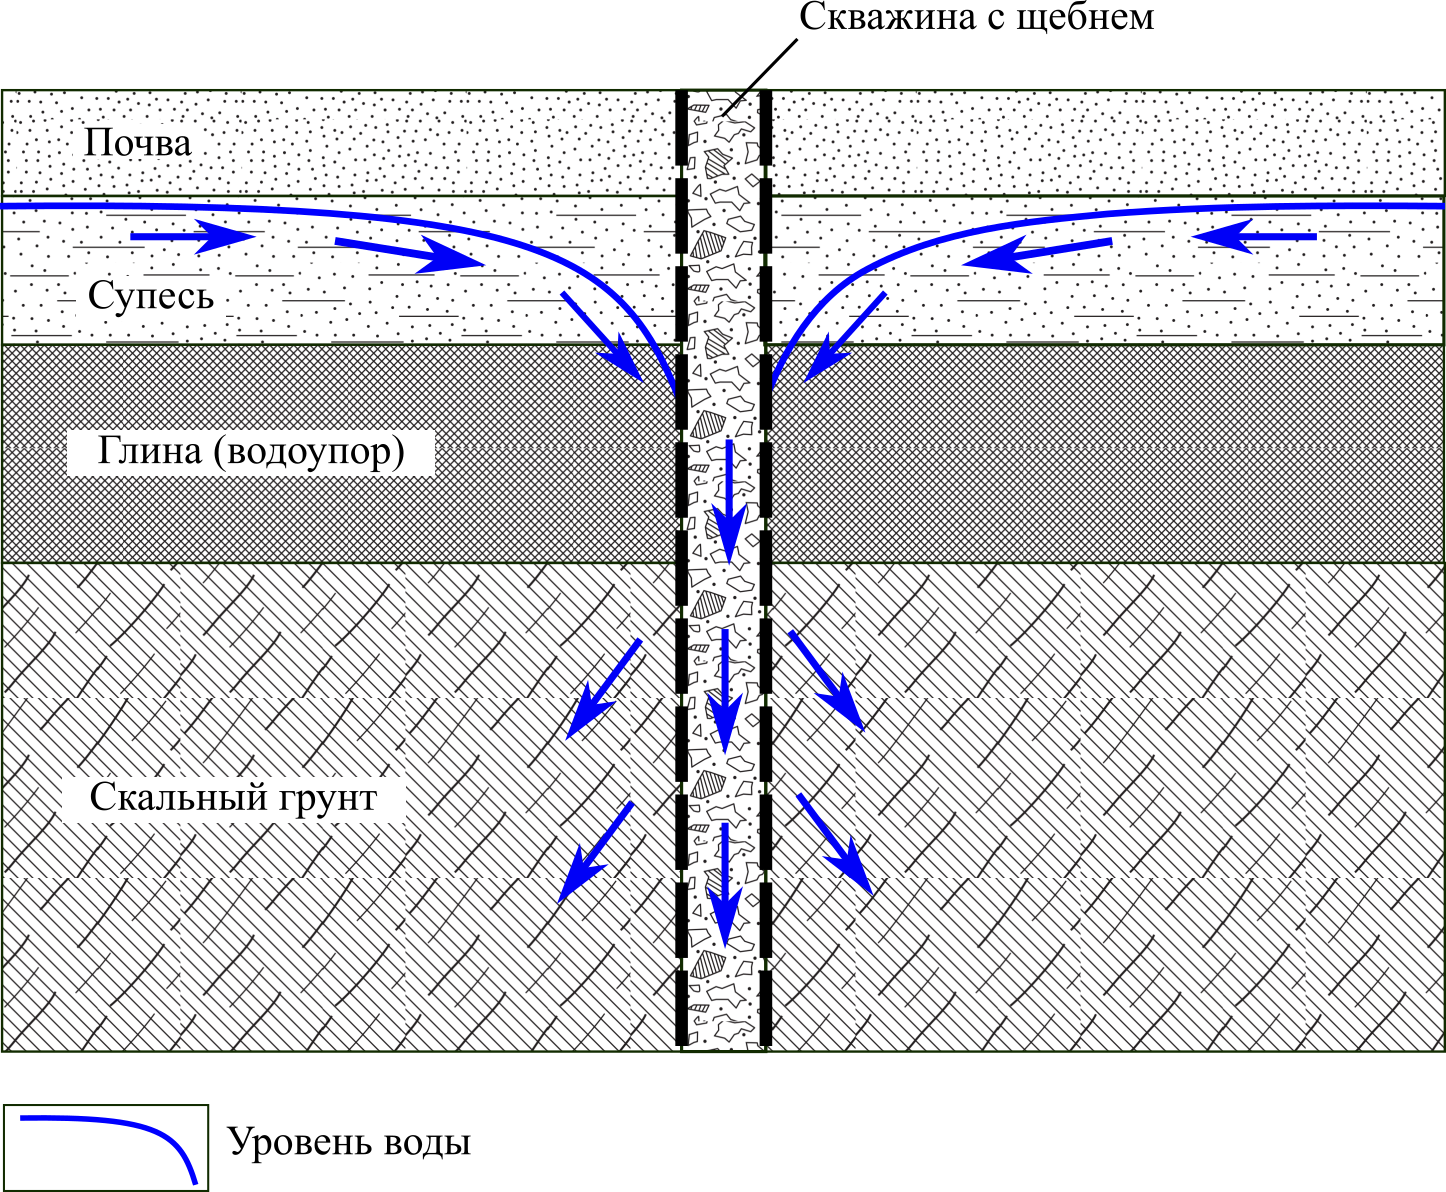
\includegraphics{img1.png}
	\caption{Схема взаимодействия двух скважин}
	\label{img:scheme2}
\end{figure}

По результатам проведенных в сходных геологических условиях в результате пробных откачек отмечается безнапорный характер подземных вод и средний дебит водопоглощающих скважин составляет $1 \, м^3/час$. Коэффициент фильтрации суглинков, залегающих в верхней части разреза, составляет 0,01 м/сут. 

При заложении групповой установки водопонижающих скважин при осушении территории скважины располагают на таком расстоянии, чтобы они влияли друг на друга, то есть расстояние между скважинами должно быть меньше радиуса влияния одиночной скважины. При этом депрессионные воронки от скважин накладываются друг на друга  и уровень воды между скважинами снижается еще больше благодаря интерференции (рис. \ref{img:scheme2}). Чем больше скважин заложено на участке осушения, тем больше снизится уровень воды в произвольно взятой точке, причем общее снижение уровня будет приближенно равно сумме снижений уровня от действия каждой скважины. Наиболее целесообразно располагать скважины на расстоянии  $0,1R$, где $R$ – радиус влияния одиночной скважины в метрах. 

На рисунке \ref{img:scheme2} изображена схема взаимодействия двух соседних скважин в групповой установке. Сплошными линиями показан уровень грунтовых вод и депрессионная воронка от каждой скважины. В результате интерференции эффективный уровень грунтовых вод показан штриховой линией. 

Глубина скважин должна быть достаточной для обеспечения необходимой водозахватной способности выбранной системы дренажа и в то же время она должна быть меньше глубины залегания подземных вод. Исходя из опыта работы авторов настоящего отчета на участках со сходными гидрогеологическими условиями, оптимальной является глубина 30 м.


\section{Определение водозахватной способности дрен}

Проверка на достаточность водозахватной способности определяется соблюдением условия:

\begin{equation}\label{eq:debit}
	Q_0 \leqslant f 
\end{equation}

	где 
	
	$Q_0$ -- дебит дрены в $м^3/сут$, 
	
	$f$ -- водозахватная способность

	\bigskip

Расчет водозахватной способности производится по формулам С.К. Абрамова для вертикальных дрен:

\begin{equation}\label{eq:abramov}
	f = 130 \pi r_c l \sqrt[3]{K}
\end{equation}

	где 

	$f$ -- водозахватная способность дрены в $м^3/сут$ на одну дрену
	
	$r_c$ -- наружный радиус вертикальных дрен, м
	
	$l$ -- длина фильтра, м
	
	$K$ -- коэффициент фильтрации водоносного пласта в $м^3/сут$
	
	\bigskip
	
	При $r_c = 0,160 \, м, l = 20 \, м, K = 0,01 \, м^3/сутки $, имеем: $f = 280 \, м^3 / сут$

	\bigskip
	
При дебите дрены $24 \, м^3/час$ условие \eqref{eq:debit} выполняется. Таким образом, \textbf{водозахватная способность дренажных скважин достаточна} для успешного водопонижения рассматриваемого участка.

\section{Выводы}

\begin{itemize}

\item Изучаемый участок сложен  трещиноватыми зелеными сланцами и амфиболитами, перекрытыми слабо водопроницаемыми суглинками и глинами с коэффициентом фильтрации $0,01 \, м^3/сут$. Грунтовые воды, приуроченные к скальным грунтам, залегают на глубинах от 30 м и имеют безнапорный характер.
\item Осложняющим фактором, вызывающим подтопление на изучаемом участке, является наличие в разрезе водонепроницаемых грунтов, сложная форма кровли суглинков и глин коры выветривания и коренных грунтов, застройка окружающей территории, что вызывает неравномерный напор приповерхностных вод.
\item Осложняющим фактором, вызывающим подтопление на изучаемом участке, является наличие в разрезе водонепроницаемых грунтов, сложная форма кровли суглинков и глин коры выветривания и коренных грунтов, застройка окружающей территории, что вызывает неравномерный напор приповерхностных вод.
\item Источником приповерхностных вод на изучаемом участке являются преимущественно атмосферные осадки и воды, образующиеся в периоды сезонного снеготаяния.
\item Поскольку устойчивые горизонты подземных вод залегают на глубинах свыше 15 м, основной причиной подтопления является отсутствие сброса собранной ливневыми желобами воды и вследствие этого, накопление ее в приповерхностных грунтах и дальнейшее ее поступление в подвальные помещения..
\item Приповерхностные воды имеют безнапорный характер.
\item Учитывая гидрогеологические условия площадки и требования к системе дренажа, был выбран вариант вертикального дренажа, представляющего собой серию из 3 водопоглощающих дренажных скважин глубиной 30 м каждая, расположенных по линии вдоль одной из стен здания (Приложение 3). Данные скважины работают как дренажно-поглощающие трубчатые колодцы - по стволам данных скважин приповерхностные воды фильтруются в водопроницаемые трещиноватые грунты, залегающие под  водоупорным горизонтом суглинков (рис \ref{img:scheme1}). За счет взаимного влияния депрессионных воронок снимаются неравномерности напора приповерхностных вод и локальные области переувлажнения несущих грунтов ликвидируются. 
\item Расстояние между скважинами и их глубины выбраны исходя из соображений баланса между эффективностью водопонижения (чем больше скважин, тем лучше) и экономической целесообразностью (чем меньше скважин, тем дешевле) и основываются в том числе на опыте работ авторов отчета на участках со сходными гидрогеологическими условиями.
\item Расчеты показывают, что водозахватная способность примененной системы дренажных скважин достаточна для успешного водопонижения рассматриваемого участка.
\item После проходки проектных 3 скважин при условии положительного эффекта планируется проходка малогабаритной буровой установкой нескольких дополнительных скважин вокруг здания (Приложение 3).

\end{itemize}

\section{Технология работ}

\begin{enumerate}
\item Для сброса дренажных вод на участке по контуру здания бурятся дренажные скважины на глубину 30 м каждая с обсадкой перфорированными полиэтиленовыми трубами.
\item В устье дренажных скважин производится выемка грунта на ширину дренажного колодца в нижней части  с расширением к верхней части. Ширина выемки в верхней части составляет 2 – 2,5 диаметра дренажного колодца. Глубина выемок 2,5 – 2,7 м. В выемках устанавливаются  дренажные колодцы (Приложение 4). Промежуток между внешними стенками дренажных колодцев и стенками выемки засыпается щебнем.
\item Дренажные колодцы закрываются крышками.

\end{enumerate}

\end{document} % конец документа

